\documentclass[preprint,12pt]{elsarticle}


%% The `ecrc' package must be called to make the CRC functionality available
%\usepackage{ecrc}

%% set the volume if you know. Otherwise `00'
%\volume{00}

%% set the starting page if not 1
%\firstpage{1}

%% Give the name of the journal
%\journalname{Expert Systems With Applications}

%% Give the author list to appear in the running head
%% Example \runauth{C.V. Radhakrishnan et al.}
%\runauth{}

%% The choice of journal logo is determined by the \jid and \jnltitlelogo commands.
%% A user-supplied logo with the name <\jid>logo.pdf will be inserted if present.
%% e.g. if \jid{yspmi} the system will look for a file yspmilogo.pdf
%% Otherwise the content of \jnltitlelogo will be set between horizontal lines as a default logo

%% Give the abbreviation of the Journal.  Contact the journal editorial office if in any doubt
%\jid{eswa}

%% Give a short journal name for the dummy logo (if needed)
%\jnltitlelogo{ESWA Logo}

%% Provide the copyright line to appear in the abstract
%% Usage:
%   \CopyrightLine[<text-before-year>]{<year>}{<restt-of-the-copyright-text>}
%   \CopyrightLine[Crown copyright]{2011}{Published by Elsevier Ltd.}
%   \CopyrightLine{2011}{Elsevier Ltd. All rights reserved}
%\CopyrightLine{2013}{Published by Elsevier Ltd.}



%\usepackage{llncsdoc}
\usepackage[figuresright]{rotating}
%\usepackage{makeidx}  % allows for indexgeneration
\usepackage{graphicx}
\usepackage[T1]{fontenc}
\usepackage[english]{babel}
\usepackage[utf8]{inputenc}
% \usepackage{multirow}

\usepackage{url}
\usepackage{rotating}

%%%Math
\usepackage{latexsym}
 \usepackage{amsmath}
% \usepackage{amssymb}
% \usepackage{amsthm}
%\usepackage{eurosans}

\usepackage{eurosym}

\usepackage{longtable}

\usepackage{listings}

\usepackage{color}
\usepackage{textcomp}


\definecolor{gray}{gray}{0.5}
\definecolor{green}{rgb}{0,0.5,0}
% 
% \usepackage{inconsolata}



\begin{document}


\begin{frontmatter}

%% Title, authors and addresses

%% use the tnoteref command within \title for footnotes;
%% use the tnotetext command for the associated footnote;
%% use the fnref command within \author or \address for footnotes;
%% use the fntext command for the associated footnote;
%% use the corref command within \author for corresponding author footnotes;
%% use the cortext command for the associated footnote;
%% use the ead command for the email address,
%% and the form \ead[url] for the home page:
%%
%% \title{Title\tnoteref{label1}}
%% \tnotetext[label1]{}
%% \author{Name\corref{cor1}\fnref{label2}}
%% \ead{email address}
%% \ead[url]{home page}
%% \fntext[label2]{}
%% \cortext[cor1]{}
%% \address{Address\fnref{label3}}
%% \fntext[label3]{}

%\dochead{}
%% Use \dochead if there is an article header, e.g. \dochead{Short communication}
%% \dochead can also be used to include a conference title, if directed by the editors
%% e.g. \dochead{17th International Conference on Dynamical Processes in Excited States of Solids}


\title{Semantic-based QoS management in Cloud Systems: Current Status and Future Challenges}


%% use optional labels to link authors explicitly to addresses:
% \author[label1]{Jose María Alvarez-Rodríguez\corref{cor1}}
% \address[label1]{The South East European Research Center, Thessaloniki, Greece.}
% \ead{jmalvarez@seerc.org}
% \ead[url]{http://www.seerc.org}
% 
% \author[label2]{José Emilio Labra-Gayo}
% \address[label2]{WESO Research Group, Department of Computer Science, University of Oviedo, 33007, Oviedo, Spain.}
% \ead{labra@uniovi.es}
% 
% \author[label3]{Alejandro Rodríguez-González}
% \address[label3]{Bioinformatics at Centre for Plant Biotechnology and Genomics UPM-INIA, Polytechnic University of Madrid, Madrid, Spain.}
% \ead{alejandro.rodriguezg@upm.es}
% 
% \author[label4]{Patricia Ordoñez De Pablos}
% \address[label4]{WESO Research Group, Department of Business Administration, University of Oviedo, 33007, Oviedo, Spain.}
% \ead{patriop@uniovi.es}





\author{}

\address{}

\begin{abstract}
The concept of Cloud Computing and Service Oriented Architectures have seen a 
dramatic increase of the amount of applications, services, management platforms, 
data, etc. gaining momentum in Information and Communication Technology and more 
specifically in the deployment of the Future Internet. However this explosion 
implies the necessity of new complex methods and techniques to deal with the 
vast heterogeneity of data sources, services or platforms. In this sense Quality 
of Service (QoS) seeks for providing an intelligent environment of 
self-management components based on domain knowledge in which both functional 
and nonfunctional properties of cloud components can be optimized in terms of 
cost, efficiency or reliability easing the transition to an advanced resource 
provisioning process. On the other hand, semantics and ontologies have emerged 
as part of the Artificial Intelligence to afford a common and standard data 
model that ease the interoperability, integration and monitorization of 
knowledge-based systems. Furthermore the Linked Data initiative as practical 
view of the Semantic Web has posed the baseline technology to easily integrate, 
enrich and consume data in a distributed system. Taking into account the 
necessity of an intelligent system to manage QoS in Cloud Systems and the 
emerging application of semantics, ontologies and Linked Data in different 
domains, this paper reviews the main approaches for semantic-based QoS 
management as well as the principal methods, techniques and standards for 
processing and exploiting diverse data providing advanced real-time monitoring 
services for QoS. A discussion of existing efforts and challenges are also 
provided to suggest future directions.
\end{abstract}

\begin{keyword}
%% keywords here, in the form: keyword \sep keyword
cloud systems \sep quality of service \sep  service oriented architectures \sep  semantics \sep  ontologies \sep  linked data \sep  sensor data \sep  big data 
%% PACS codes here, in the form: \PACS code \sep code

%% MSC codes here, in the form: \MSC code \sep code
%% or \MSC[2008] code \sep code (2000 is the default)

\end{keyword}


\end{frontmatter}

\section{Introduction}
Cloud Computing~\cite{mell2011nist} systems and Service Oriented Architectures (SOA) have 
reached a level of complexity~\cite{Huebscher:2008:SAC:1380584.1380585,Conejero:2012:MSQ:2357487.2357591} that implies the necessity of new methods 
and algorithms to automatically deal with the vast amount of data, variables, 
parameters, etc. that appear in this new realm for the advanced management of 
applications, services or resources. 

In this new environment QoS is playing a relatively minor role but its 
importance, in a wide range of applications scenarios, is likely become more 
crucial than ever before. In recent years and due to the deployment of web 
services a considerable research effort in QoS has been made. However existing 
QoS mechanisms are actually available in a few large scale commercial 
environments and with a limited extent. The main problem lies in the complexity 
of designing QoS models that enables an adequate management of a distributed 
architecture making decisions about resource provisioning, getting feedback for 
the final users, etc. with the objective of avoiding existing ``brute-force''
solutions and overprovisioning. 

Although QoS management has been also widely investigated~\cite{Conejero:2012:MSQ:2357487.2357591} 
in the well-known grid-computing area the emergence of the Cloud Computing paradigm 
brings a new set of open issues: accomplish the  Service Level Agreements (SLAs), predict 
future workload, process large and diverse data streams/logs, make real-time 
decisions, reasoning and inference, dynamic adaptation and provision of 
resources, etc. In the widely-accepted definition~\cite{mell2011nist} of 
he National Institute of Standards and Technology (NIST) QoS 
would be aligned to the concept of ``Measured Service'', see Figure~\ref{fig:qos-intro}, and 
more specifically to define both characteristics applicable to a service and operations 
to deliver some kind of alert or predictive analytics service. 
The aforementioned points are very challenging and should be 
addressed in order to ease an intelligent, flexible and self-managing system of 
cloud-based applications and platforms.


 \begin{figure}[!ht]
\centering
	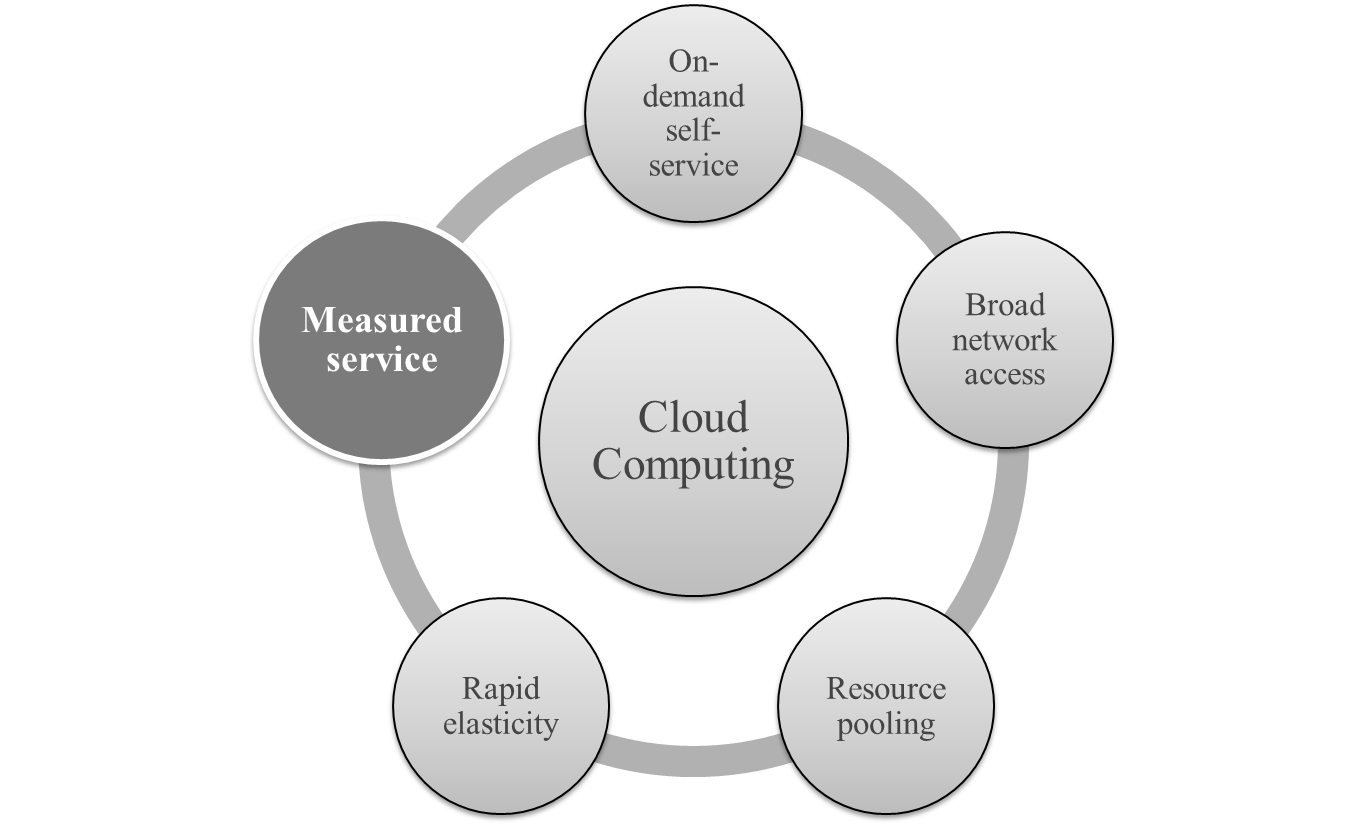
\includegraphics[width=12cm]{./imgs/qos-intro}
 \caption{Quality of Service in the NIST definition~\cite{mell2011nist}.}
 \label{fig:qos-intro}
\end{figure}

Furthermore a proper management of a cloud system taking into account QoS 
features can save costs, keep high-performance, reserve resources on-demand and 
offer a user-friendly experience to both IT managers and final users. 
Traditionally, QoS has been handled using a combination of network resource 
provisioning with techniques such as admission control or active queue 
management. Nowadays these old-fashioned techniques can be applied to a static 
environment but in the future, the challenge of providing higher elasticity and 
dynamic adaptation cannot be accomplished with these methods. In this sense it 
is clear that QoS will remain a fundamental requirement in the next wave of 
applications and services on the Web and there is no doubt that QoS should 
address the new challenges applying emerging and trending technology and 
approaches to overcome existing restrictions in QoS models.

The features and requirements of these new cloud systems with regards 
to QoS~\cite{Pedersen:2011:AMQ:2114495.2115542} match the advantages of software component and 
knowledge-based architectures. In fact, Autonomic Computing support for the next generation of cloud systems 
needs to be~\cite{Conejero:2012:MSQ:2357487.2357591,Pedersen:2011:AMQ:2114495.2115542}: 
1) Self-x management, 2) agile, flexible and reliable, 4) deployable over a multiple cloud platforms, 5) handle complexity, 6) enable 
collaboration and coordination and 7) cost-effective and greener 
(energy-efficient). Under this context, semantic technologies have emerged as an 
option to design and develop intelligent software components and agents to 
perform certain tasks on the Web and fulfill user's requirements (in this case 
applications). Therefore, Semantics enables machines to automatically process 
and enrich data from different sources and has the potential to deeply influence 
the further development of the Internet Economy as cloud systems also does.

In the Semantic Web area, there is a growing commitment to process large data streams applying 
new stream reasoning~\cite{Bolles:2008:SSE:1789394.1789438,Barbieri:2010:EEC:1739041.1739095} 
or complex event processing (CEP) techniques~\cite{Anicic:2011:EUL:1963405.1963495}. Furthermore there are research works offering cloud-based 
solutions to deal with Big Data~\cite{Fan:2013:MBD:2481244.2481246} (e.g. analysis of social media), modeling SLAs and ECA rules with ontologies, 
monitoring real-time systems (e.g. traffic), sensor networks, or making decisions in a collaborative fashion~\cite{RodriGuez-GonzaLez:2012:UAP:2350799.2350907} (e.g. clinical reasoning). 
The main advantage of applying semantic technologies to a specific domain lies in the standard representation of knowledge and data through a common-shared data model (RDF) and the 
capacity of reusing existing knowledge through ontologies (OWL). Thus, data coming from cloud systems can be automatically processed, checked for inconsistencies and 
used in expert systems to support self-x management activities.

This review is intended to provide researchers, developers and practitioners a summary of the current status of QoS management in Cloud Computing and SOA applying semantics. To do so, the paper 
is structured as follows. Next section reviews the background concepts required to a better understanding of the paper. Section~\ref{qos-semantics} 
presents the existing works to perform QoS management using semantics; more specifically most of the ontology-based frameworks for 
QoS management are reviewed. Afterwards, a review of existing techniques for processing large data streams is also provided in Section~\ref{data-stream}. 
Section~\ref{framework} outlines a framework to meet QoS requirements applying semantics and data strea processing techniques in real-time. 
Finally, the paper ends with an evaluation, discussion of existing approaches for semantic-based QoS management, 
limitations, future challenges and concluding remarks. 


% \section{Literature Review}\label{sect:related-work}
% 
% \section{Evaluation}\label{sect:evaluation}
% 
% \section{Conclusions and Future work}\label{sect:conclusions}
% 
% \nocite{*}
\bibliographystyle{plain}
% %\bibliographystyle{unsrt}
% % %\bibliographystyle{acm}
\bibliography{cloud-references}
 % \renewcommand{\bibname}{References}


\end{document}
